%%%%%%%%%%%%%%%%%%%%%%%%%%%%%%%%%%%%%%%%%
% Thin Sectioned Essay
% LaTeX Template
% Version 1.0 (3/8/13)
%
% This template has been downloaded from:
% http://www.LaTeXTemplates.com
%
% Original Author:
% Nicolas Diaz (nsdiaz@uc.cl) with extensive modifications by:
% Vel (vel@latextemplates.com)
%
% License:
% CC BY-NC-SA 3.0 (http://creativecommons.org/licenses/by-nc-sa/3.0/)
%
%%%%%%%%%%%%%%%%%%%%%%%%%%%%%%%%%%%%%%%%%

%----------------------------------------------------------------------------------------
%	PACKAGES AND OTHER DOCUMENT CONFIGURATIONS
%----------------------------------------------------------------------------------------

\documentclass[a4paper, 11pt]{article} % Font size (can be 10pt, 11pt or 12pt) and paper size (remove a4paper for US letter paper)
\usepackage[inner=2cm,outer=2cm]{geometry} %left=4cm,right=2cm would be equivalent

\usepackage[protrusion=true,expansion=true]{microtype} % Better typography
\usepackage{graphicx} % Required for including pictures
\usepackage{wrapfig} % Allows in-line images
\usepackage{subfigure}
\usepackage{amsmath}
\usepackage{mathpazo} % Use the Palatino font
\usepackage[T1]{fontenc} % Required for accented characters
\usepackage[titletoc,page]{appendix}
\newcommand{\sqlen}[1]{\ensuremath{(x - x_{#1})^2 + (y-y_{#1})^2}}
\newcommand{\rili}[1]{\ensuremath{\frac{r_{#1}^2}{l_{#1}}}}
\usepackage[mediumspace,mediumqspace,Grey,squaren]{SIunits}
\linespread{1.05} % Change line spacing here, Palatino benefits from a slight increase by default

\makeatletter
\renewcommand\@biblabel[1]{\textbf{#1.}} % Change the square brackets for each bibliography item from '[1]' to '1.'
\renewcommand{\@listI}{\itemsep=0pt} % Reduce the space between items in the itemize and enumerate environments and the bibliography

\renewcommand{\maketitle}{ % Customize the title - do not edit title and author name here, see the TITLE block below
\begin{flushright} % Right align
{\LARGE\@title} % Increase the font size of the title

\vspace{50pt} % Some vertical space between the title and author name

{\large\@author} % Author name
\\\@date % Date

\vspace{40pt} % Some vertical space between the author block and abstract
\end{flushright}
}

%----------------------------------------------------------------------------------------
%	TITLE
%----------------------------------------------------------------------------------------

\title{\textbf{Constrained Constructive Optimization implementation}\\ % Title
Reproducing Rudolph Karch paper} % Subtitle

\author{\textsc{Clara Jaquet} % Author
\\{\textit{Paris-Est University}}} % Institution

\date{\today} % Date

%----------------------------------------------------------------------------------------

\begin{document}

\maketitle % Print the title section

%----------------------------------------------------------------------------------------
%	ABSTRACT AND KEYWORDS
%----------------------------------------------------------------------------------------

%\renewcommand{\abstractname}{Summary} % Uncomment to change the name of the abstract to something else

\begin{abstract}
This report aims to explain the CCO algorithm implementation in 2D, and its 3D extension. This algorithm has been detailed by Schreiner in 2D \cite{schreiner1993computer} and Karch in 3D \cite{karch1999three}. Because the implementation principle is spread between several articles, we propose to summarize hereafter the whole implementation. Along the way, we provide our own interpretation of some finer details of the method, that leave room for variants.
%This report aims to explain the CCO implementation in 2D then 3D, based on Karch's work \cite{karch1999three}.
%For efficiency purpose, the encapsulated articles contained in this work requires
%to be summarized in one paper.
 
The CCO algorithm combines computational fluid dynamics laws, network geometry and topology optimization to mimic vascular network growth.

%In a future step we will consider the implementation for non convex volumes, extension provided by Schreiner \cite{schreiner2006optimized}.

\end{abstract}

\hspace*{3,6mm}\textit{Keywords:} constrained constructive optimization, implementation % Keywords

\vspace{30pt} % Some vertical space between the abstract and first section

\tableofcontents
%----------------------------------------------------------------------------------------
%	ESSAY BODY
%----------------------------------------------------------------------------------------

\section*{Introduction}

Constrained Constructive Optimization (CCO) consists of growing a tree governed by minimizing a target function. 

In Karch's method the tree is constrained into a growing convex perfusion volume, and the target function minimizes the total tree volume. Segments are added one by one and subjected to both local optimization (single bifurcation scale) and global optimization (tree scale). The local optimization is based on Kamiya's work \cite{kamiya1972optimal}, whereas the global tree optimization has been implemented first by Schreiner in 2D \cite{schreiner1993computer}. 

\section{Global tree optimization}

Initialization of the method requires as input some physiological parameters, the number of terminal segments to reach, and a randomized starting point.


The CCO algorithm is introduced with the organigram in figure \ref{fig:algo loop}.
\begin{figure}[htbp]
\centering
\subfigure{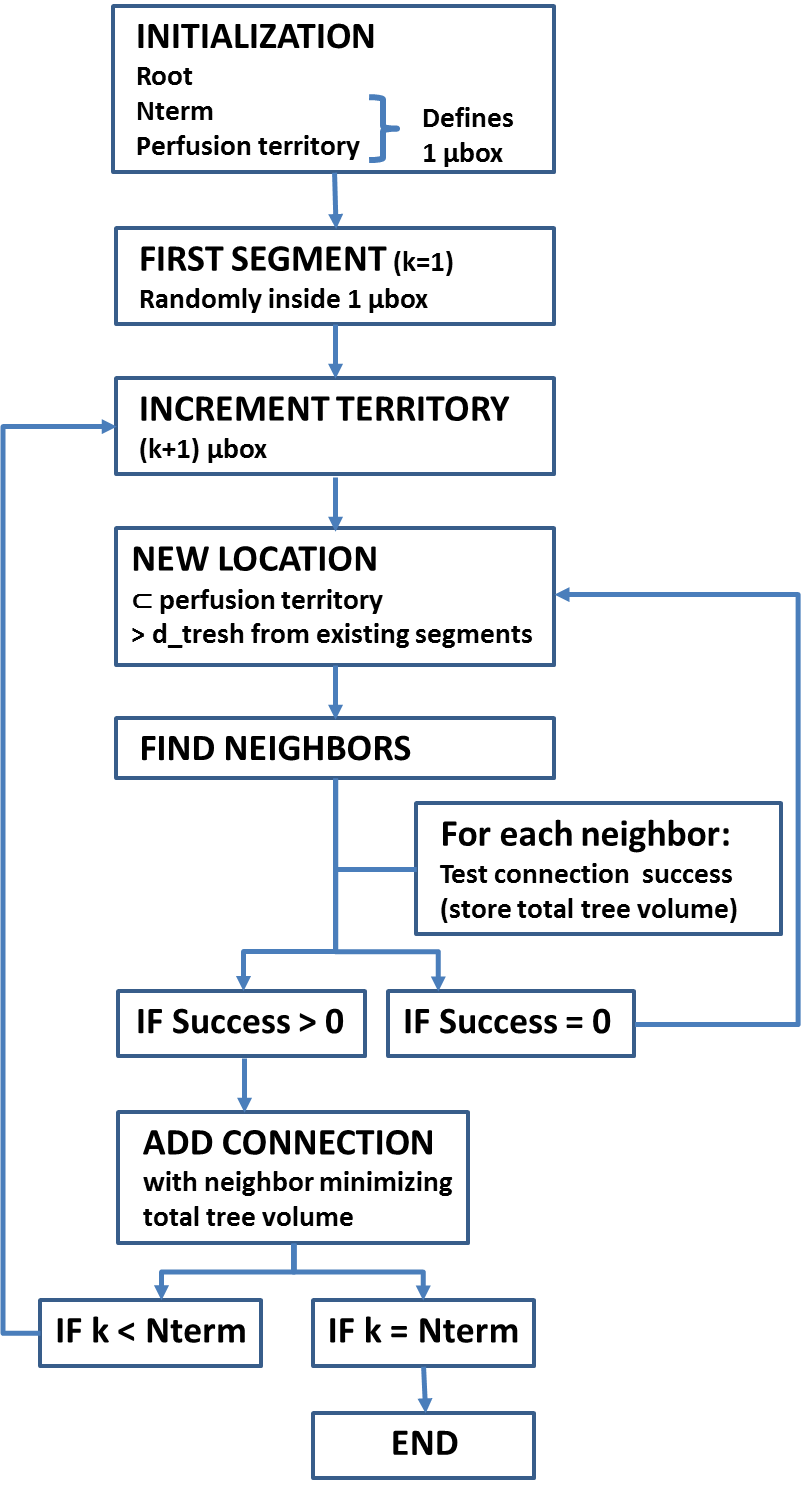
\includegraphics[width=0.4\textwidth]{./Images/AlgorithMainLoops.png}}
\caption{Algorithm of CCO. ${d\_tresh}$ is a distance threshold calculated at each iteration. A microbox corresponds to an average area per terminal segment.}
\label{fig:algo loop}
\end{figure}


Each loop of the algorithm determines a new segment to be added onto the tree. Figure \ref{fig:algo illustr} provides an example of the result of the first three loops.
\begin{figure}[htbp]
\centering
\subfigure{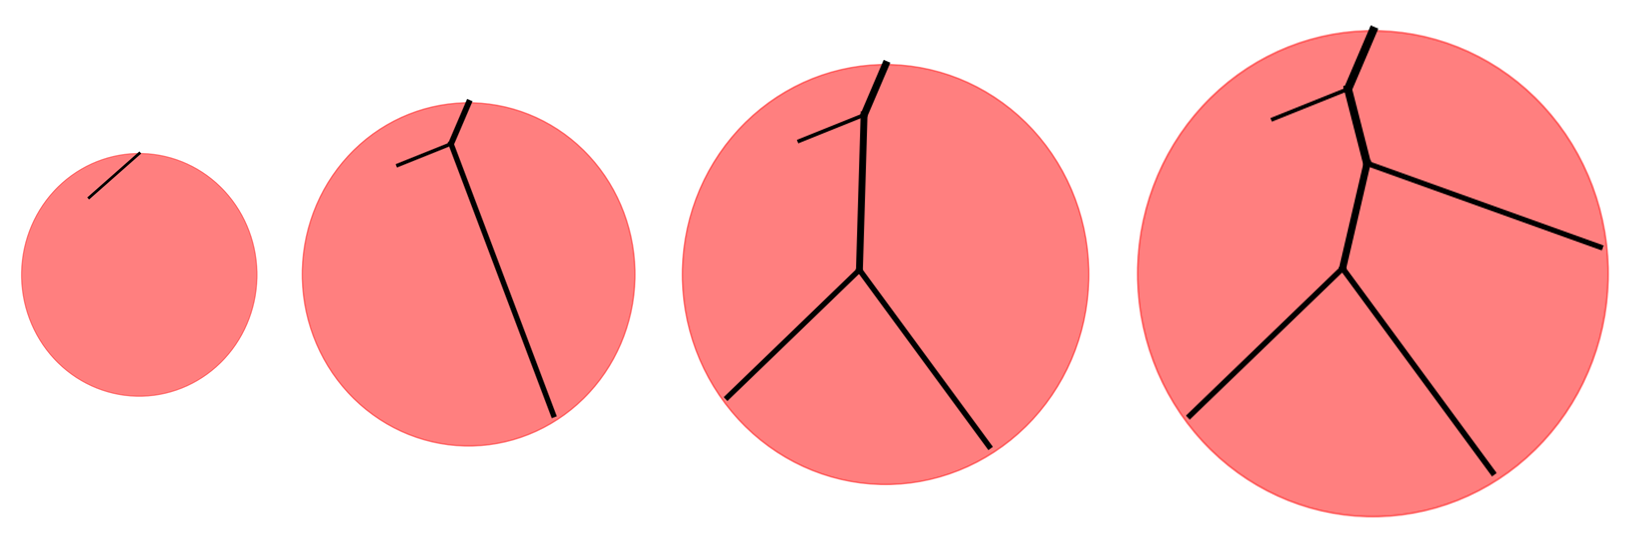
\includegraphics[width=0.5\textwidth]{./Images/ExampleTreeGrowth.png}}
\caption{CCO example : output images of the first three loops.}
\label{fig:algo illustr}
\end{figure}
The perfusion territory is slightly increased before each new added segment, to simulate tissue growth concomitant with vascular growth.
% to increment the tree of a new segment after a whole 
% consists of a complete loop for each added segment. 
A  random location is picked under some constraints (geometrical and physiological), to use it as a candidate for segment extremity. Its connection is tested with neighbor segments, producing a bifurcation under topological, structural and functional constraints.
Due to mechanical laws, each connection also induces a specific adjustment of all existing segment diameters. The optimal connection is then selected among all connections as the one minimizing a target function (the minimal volume of the total tree).
% In view of this new branch impact on the whole tree (induced by fluid mechanics laws), the optimal connection is selected by minimizing a target function (the minimal volume of the total tree). 




\subsection{Assumptions and boundary conditions}
The vascular tree grows under specific assumptions and boundary conditions.

The perfused volume is supposed convex and homogeneously filled. The terminal segments correspond to pre-arteriole level, feeding a non modeled micro-vasculature.
The blood is an incompressible, homogeneous Newtonian fluid, studied in a steady state and in laminar flow conditions. 

The resistance and the pressure drop of a segment $j$ are defined by:
\begin{equation}\label{resistance}
R_j = \frac{8\mu}{\pi}\frac{l_j}{r_j^4} \text{ with } \mu \text{ the viscosity }
\end{equation}
\begin{equation}\label{Pdrop}
\Delta P_j = R_j Q_j
\end{equation}
The total resistance of the tree is calculated recursively by tree decomposition, considering parallel and serial arrangements.

The physiological parameters are set following table \ref{tbl:toto}:\\ % missing table
\begin{table}
\begin{center}
\begin{tabular}{ccc}

\hline

Parameter & Meaning & Value\\
\hline
$V_{perf}$ & perfusion volume   & \unit{100}{\centi\cubic\meter}\\
$P_{perf}$ & perfusion pressure & \unit{100}{\milli\meter}Hg\\
$P_{term}$ & terminal pressure  & \unit{60}{\milli\meter}Hg\\
$Q_{perf}$ & perfusion flow     & \unit{500}{\milli\liter / \min}\\
$Q_{term}$ & terminal flow 	    & \unit{0.125}{\milli\liter / \min}\\
$N_{term}$   & number of terminals & 4000\\
$\mu$	   & viscosity of blood & \unit{3.6}{\centi}p\\
$\gamma$   & Murray bifurcation exponent & 3\\
\hline
\end{tabular}
\end{center}
\caption{Global model parameters}
\label{tbl:Global model parameters}
\end{table}


The pressures at distal end of terminal segments, $P_{term}$, are equal and correspond to the inflow pressure to the micro-circulation.

The terminal flows $Q_{term,j}$ are equal, and delivered into the micro-circulation against $P_{term}$. Because of flow conservation, the $Q_{term,j}$ sum corresponds to the perfusion flow at the root $Q_{perf}$. 

The laminar flow resistance of the whole tree induces a given total $Q_{perf}$ accross the overall pressure drop $\Delta P$. 
%The perfusion flow $Q_{perf}$ is the same for each step of the tree generation.

The produced tree is binary and its total number of segments is calculated from:
\begin{equation}
N_{tot} = 2 N_{term} -1
\end{equation}

This tree is subjected to Murray's law, with a power coefficient equal to 3.

\subsection{Initialization step}  
Inputs:
\begin{itemize}
\item convex perfusion surface ($A_{perf}$) or volume ($V_{perf}$) definition: position and shape. In our case we work within simple shapes: circular or spherical shape.
\item number of terminal segments, $N_{term}$
\item location of the root (in our case on the border of the perfusion territory)
\item a random location inside the perfusion territory for the end of the first segment 
\end{itemize}

From these inputs we estimate the average perfusion territory of each terminal segment when reaching the goal $N_{term}$, named "micro-circulatory black-box" \cite{schreiner1993computer}. We calculate $r_{supp}$, the average radius of the black-boxes:
\begin{equation}
\pi r_{supp}^2 = A_{perf} / N_{term}
\label{eq rsupp2D}
\end{equation}  

Before adding a segment, the perfusion territory area is incremented of one micro-circulatory black-box. So, calling $k_{term}$ the number of terminal segments at the current step of the algorithm, we obtain after the inflation the perfusion territory area $A_k$:
\begin{equation}
A_k = (k_{term} + 1) \pi r_{supp}^2
\end{equation}

The segments are stretched correspondingly to this inflation. First their new lengths are calculated, then each segment radius is rescaled in order to adapt the new tree resistance. 
Note that we do not recalculate segment positions after tree stretching but compute a conversion to the $k_{world}$ via a scaling factor $r_{kf}$:
\begin{equation}
r_{kf} = \sqrt{\pi A_k}
\end{equation}   
%With this factor applied on segment length, we recalculate all segment resistances via a depth-first algorithm. Segment radii are consequently rescaled to adapt the new resistances.
The tree is adjusted to the inflated world before starting the loop to add a new segment.

In a similar fashion, knowing the flow at terminal segments $Q_{term}$, we will increase the perfusion flow with each during the loop to add a new segment, calculating as:
\begin{equation}
Q_{pk} = k_{term} Q_{term}
\end{equation}  




\subsection{Loop to add new segment}
We are provided a new location, $n_{loc}$, and want to find its optimal connection to the existing tree. For this purpose we select the $N_{con}$ closest existing segments to this location, test their optimal connection to the new location, and store the total tree volume resulting of it. Then, as a global optimization process, we select the neighbor connection best minimizing the total tree volume.


%compute a local optimization for each of them, then evaluate the connection impact on the whole tree, and as a global optimization process, we determine the one minimizing best the total tree volume.

\begin{figure}[!h]
\centering
\subfigure{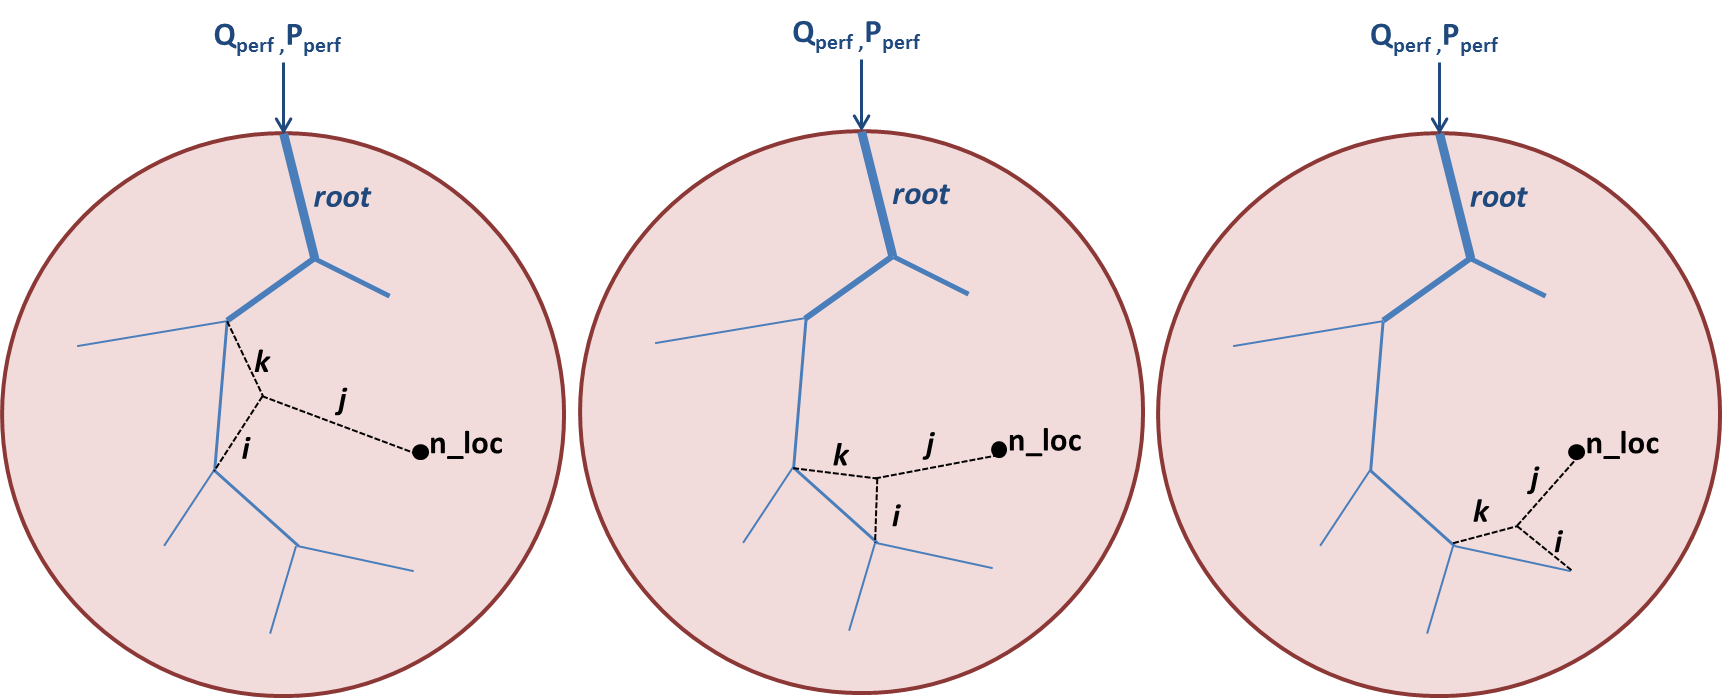
\includegraphics[width=0.9\textwidth]{./Images/AddNewSegmentTestNeighbors.png}}
\caption{To add a new segment: test connection with neighbors of the new location $n_{loc}$}
\label{fig:test neighbors}
\end{figure}

\subsubsection{Constrained new location $n_{loc}$}
A random position is picked, that has to fulfill two constraints: belonging to the perfusion territory and respecting a distance criterion. 
This criterion is defined based on the final and current size of the tree. In 2D, it is given by the following equation:
\begin{equation}
d_{thresh} = (\pi r_{supp}^2 / k_{term})^\frac{1}{2}
\end{equation}
with $r_{supp}$ calculated from equation (\ref{eq rsupp2D}).%with $k_{term}$ the number of terminal segment at the current step.
%, and $r_{supp}$ defined from  the estimated size of a micro-circulatory black-box area, knowing the total perfused area $A_{perf}$:
%\begin{equation}
%\pi r_{supp}^2 = A_{perf} / N_{term}
%\end{equation}

In 3D this criterion is defined as:
\begin{equation}
d_{thresh} = (\frac{4}{3} \pi r_{supp}^3 / k_{term})^\frac{1}{3}
\end{equation}
with
\begin{equation}
\frac{4}{3}\pi r_{supp}^3 = V_{perf} / N_{term}
\end{equation}
This distance criteron is updated after each new segment is added, so that it decreases during tree growth. If no location is found (after $max\_trial = 1000$) that respects this distance to existing segments within the perfusion territory, then the distance criterion is multiplied by 0.9 and the process repeated until a new position is found that fulfills both constraints. 

\subsubsection{Test connection}

The connection test corresponds to a single bifurcation optimization while taking into account its impact on the whole tree.\\

Kamiya proposes a single bifurcation optimization by an iterative procedure \cite{kamiya1972optimal}, which is fully detailed in section \ref{Kamiya}. 
At each of Kamiya's iteration, we are provided a bifurcation point location and radii of the concerned segments. 
\begin{enumerate}
\item  We control that the resulting segments are not degenerate, which means all three segments of the new bifurcations respect the following constraint between length and radius: $2r_i \leq l_i$. If they do degenerate we consider this bifurcation non plausible, skip it, and go to testing another neighbor segment.

\item We assess and apply the consequence of this connection on the whole tree before measuring the total tree volume. This process is detailed in sections \ref{propagate} and \ref{target}.

\item We calculate the total tree volume gradient (relative to the previous result of Kamiya iteration).
Along Kamiya's iterations, the total tree volume is expected to converge to a local minimum. The convergence is determined with a tolerance empirically fixed (in our case $tolerance = 0.01$). 

\end{enumerate}

 
If the convergence is reached, we apply an additional checks: we control that none of the three resulting segments overlap any other existing tree segment.
The bifurcation location, segments radii, and total tree volume at convergence are stored to be later compared with other connections.

If the convergence has not been reached yet, we set the current radii and point location as a new starting point for Kamiya's optimization search.

%Calculating the volume gradient along each iteration,  
%If the iteration is successfull, (it can fail because induces convergence research), we use 


%For each neighbor segment of $n_{loc}$ we calculate what would be the optimal connection to $n_{loc}$ based on a single bifurcation optimization procedure established by Kamiya \cite{kamiya1972optimal}, and is fully detailed in section \ref{Kamiya}. If this local optimization process is successful, we apply two additional checks:
%\begin{itemize}
%\item We control that the resulting segments are not degenerate, which means all three segments of the new bifurcations respect the following constraint between length and radius: $2r_i \leq l_i$
%
%\item We control that none of the three resulting segments overlap any other existing tree segment.
%\end{itemize}
%
%With this step we ensure the connection to be locally optimal and plausible for the tree.

\subsubsection{Propagate new bifurcation impact on the whole tree}
\label{propagate}
By adding a new terminal segment, generating a new bifurcation, we perturb the distribution of segmental flows. In order to reestablish the correct terminal flows, the hydrodynamic resistance of the tree must be adjusted. As the lengths of the segments as well as the terminal and perfusion pressures are fixed, this can only be accomplished by proper rescaling of the segment's radii.\\

If we define the reduced hydrodynamic resistance $R^*$ as $R^*_i = R_i r_i^4$ we can calculate the reduced hydrodynamic resistance of a segment including its left and right subtrees by recursively traversing the subtrees:
\begin{equation} \label{red resistance}
R^*_{sub,j} = \frac{8\mu}{\pi}l_j + \left( \frac{(r_{left,j}/r_j)^4}{R_{left,j}^*} + \frac{(r_{right,j}/r_j)^4}{R_{right,j}^*}\right)^{-1}
\end{equation}
Considering the equations \eqref{Pdrop} and \eqref{resistance}, we can calculate the radius ratio of two children segments from resistance and flow:
\begin{equation} \label{children ratio}
\frac{r_i}{r_j} = \left(\frac{Q_iR_{sub,i}^*}{Q_jR_{sub,j}^*}\right)^\frac{1}{4}
\end{equation}
with $Q_i$ and $Q_j$ the respective flow of sibling segments $i$ and $j$.

Instead of storing the absolute radius for each segment, we consider the ratio between parent and its children: $\beta^i_k = r_i / r_k$ and $\beta^j_k = r_j / r_k$ with i and j the children, k the parent segment. Since the tree respects Murray's law, these ratios can actually be calculated directly from the ratio between children segments (see appendix \ref{appendix:1} for details):
\begin{equation}
\beta^i_k = \left( 1 + (\frac{r_i}{r_j})^{-\gamma}\right)^{-\frac{1}{\gamma}} \text{ and }
\beta^j_k = \left( 1 + (\frac{r_i}{r_j})^{\gamma}\right)^{-\frac{1}{\gamma}}
\end{equation}


Calculating the reduced resistance for each children with \eqref{red resistance}, and knowing the flow, we obtain the children radius ratio from \eqref{children ratio}, which is used to calculate the $\beta$ values, stored with the parent segment properties. 
The subtrees distal to the new bifurcation remain constant and unaffected by the addition of the new branch, whereas upstream bifurcations are updated following this exact same process. By this method, called "balancing of bifurcation ratios", radius rescaling is propagated up the tree.
 


\subsubsection{Measure target function}
\label{target}
Calculate the root radius from
\begin{equation}
r_{root} = \left( R_{sub, root}^* \frac{Q_{pk}}{P_{perf}-P_{term}}\right)^\frac{1}{4}
\end{equation}
Then for each segment we obtain the radius from:
\begin{equation}
r_i = r_{root} \prod\limits_{k=i}^{root} \beta_k
\end{equation}

So we can calculate the total tree volume. This is the target function that we seek to minimize:
\begin{equation}
T_i = l_i^{\mu} r_i^{\lambda}
\end{equation}

 

\subsubsection{Select best connection between neighbors}
We store the target function result in the Connection Evaluation Table (CET), for each of the tested neighbor connection. The connection yelding the lowest total tree volume is considered as the optimal one and added to the tree, updating flows and resistances.

If the CET does not contain at least two plausible connections among the $N_{con} = 20$ neighbors tested, then we extend the search to the $N_{max} = 40$ neighbor segments. If at least two plausible connections still do not come out of this process, we reject the tested location $n_{loc}$ and start again the main loop to add a new segment with a new random location.
By plausible connection we mean the local optimization converges, with no degenerate segment and no crossing of any other tree segment. 


\subsection{Example of results and comparison}
When comparing image results of our simulated 4000 $N_{term}$ tree, figure \ref{fig:CCO 2D}, with Schreiner's results \cite{schreiner1993computer},see figure \ref{fig:Schreiner result}, it seems we do not obtain the same radii. 
\begin{figure}[htbp]
\centering
\subfigure{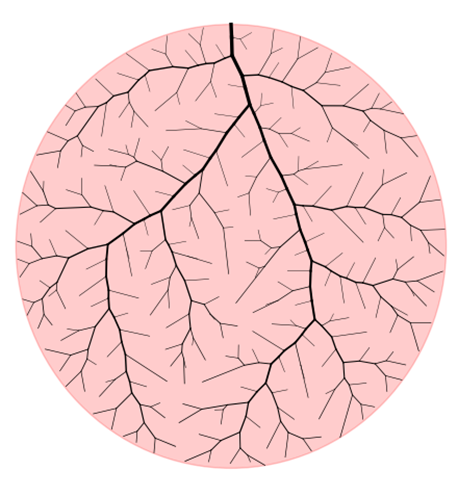
\includegraphics[width=0.45\textwidth]{./Images/CCOResults/tree_Nt250_s42_33.png}}
\subfigure{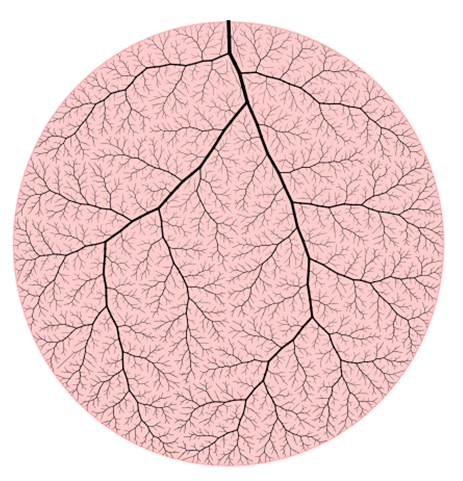
\includegraphics[width=0.45\textwidth]{./Images/CCOResults/tree_Nt4000_s42_33.png}}
\caption{Output of CCO in 2D with different $N_{Term}$. (left) A $250 N_{term}$ tree generated in \unit{9}{min}. Note:The terminal pressure is adapted to the number of terminal segments, $P_{term}$=\unit{63}{\milli\meter}Hg. (right) A $4000 N_{term}$ tree generated in 33 hours.}
\label{fig:CCO 2D}
\end{figure}
\begin{figure}[htbp]
\centering
\subfigure{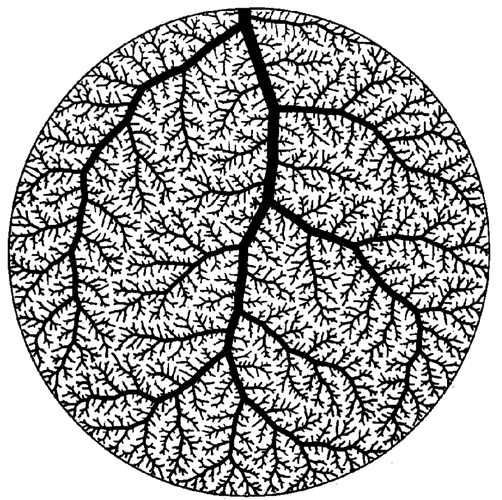
\includegraphics[width=0.45\textwidth]{./Images/CCOResults/SchreinerResult.png}}
\caption{Fig 3 from Schreiner \cite{schreiner1993computer} : $4000 N_{term}$ tree.}
\label{fig:Schreiner result}
\end{figure}

Actually, this visual difference might be due to their visualization tool resolution, that could be limited.
Such assumption seems coherent when comparing the measured radii on $250 N_{term}$ tree along bifurcation levels, cf figure \ref{fig:Schreiner radii study}. 

Schreiner computed these 10 tree models with a Murray coefficient $\gamma =2.55$. In figure \ref{fig:Schreiner radii study} right, we provide the same study with different gamma values. Our curve for $\gamma = 2.55$ is pretty similar to Schreiner result, except that the slope is slightly steeper at the beginning. Also, our mean diameter tends to 0.5mm when reaching the 35th bifurcation level.


\begin{figure}[htbp]
\centering
\subfigure{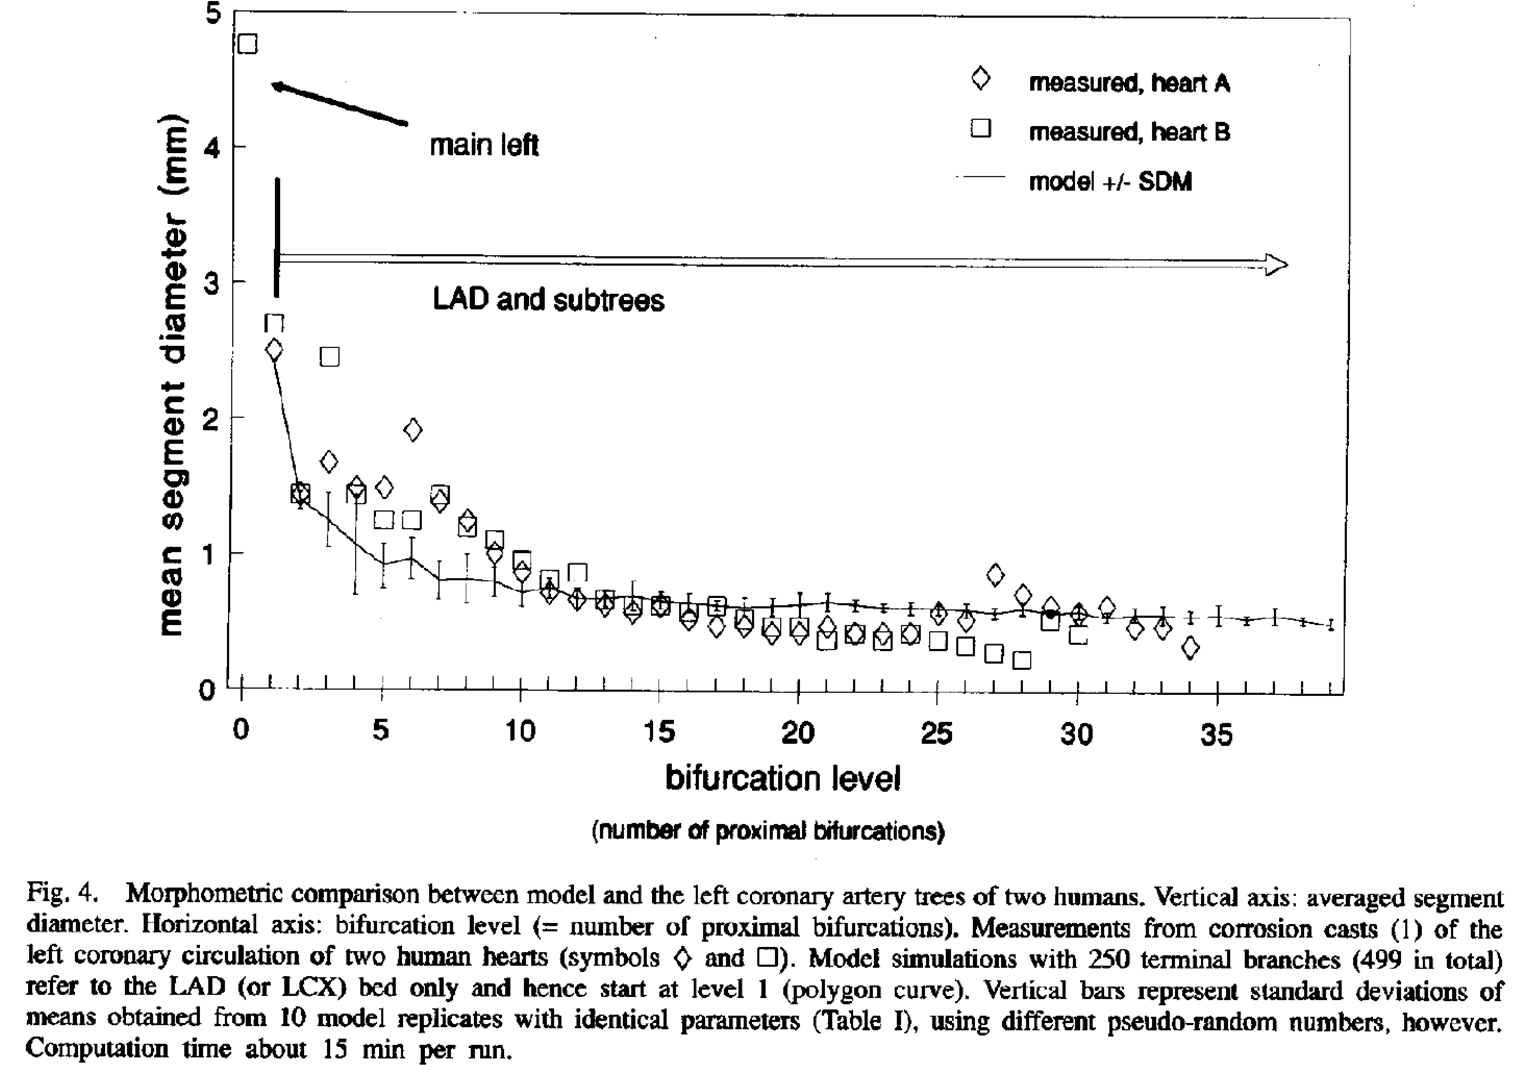
\includegraphics[width=0.66\textwidth]{./Images/CCOResults/SchreinerRadiiResult250Nt.png}}

\subfigure{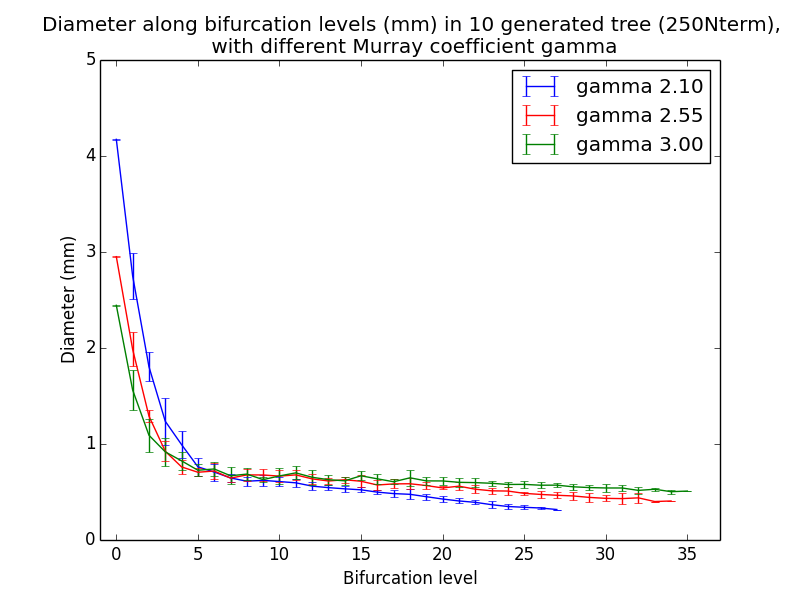
\includegraphics[width=0.52\textwidth]{./Images/CCOResults/DiamAlongBif_Nt250_seeds33to43_gammacomparison.png}}
\caption{Radius study along bifurcation levels: mean and standard deviation at each bifurcation level on 10 simulated trees. Top: result from Schreiner \cite{schreiner1993computer}, including simulated model and measured radii on anatomical data, computed with $\gamma = 2.55$. Bottom: our result comparing $\gamma$ values: $2.1, 2.55$ and $3.0$.}
\label{fig:Schreiner radii study}
\end{figure}


If we compare our 2D CCO radii distribution with Karch results (computed in 3D), in figure \ref{fig:Karch radii study} we have similar mean variations, in particular the slope steepness along the first bifurcation levels.
\begin{figure}[htbp]
\centering
\subfigure{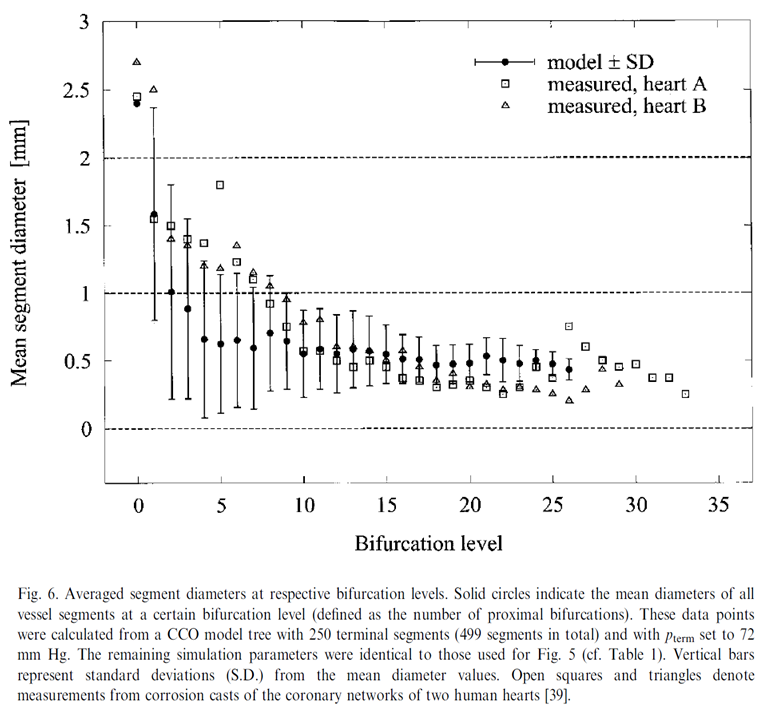
\includegraphics[width=0.6\textwidth]{./Images/CCOResults/KarchRadiiResult250Nt.png}}
\subfigure{\includegraphics[width=0.494\textwidth]{./Images/CCOResults/DiamAlongBif_Nt250_over10trees_M300_PK_seeds35only.png}}
\subfigure{\includegraphics[width=0.494\textwidth]{./Images/CCOResults/DiamAlongBif_Nt250_over10trees_M300_PK_seeds36only.png}}
\caption{Radius study along bifurcation levels: mean and standard deviation at each bifurcation level on 1 single simulated 250Nterm tree. Top: result from Karch on 3D CCO \cite{karch1999three}, including simulated model and measured radii on anatomical data, computed with $\gamma = 3.0$. Bottom: our result computed on two trees from 2D CCO, with same $\gamma$ value.}
\label{fig:Karch radii study}
\end{figure}

The algorithm we implemented might not be exactly the same as Karch and Schreiner,due to internal parameters that were not detailed in their work, such as:
\begin{itemize}
\item $d\_tresh$ adaptation: we decrease $d\_tresh$ of $10\%$ after 1000 unsuccessful iterations to get a new location inside perfusion territory far enough from existing segments. There are no precision, neither in Schreiner nor Karch work about this boundary.
\item convergence boundary: we consider reaching convergence when total tree volume gradient between iterations is below \unit{0.01}{\milli\cubic\meter}, and should be reached before 100 Kamiya's iterations.
\end{itemize}
Nonetheless, by comparing results, visually and quantitatively (radii study), we can assume we produced a similar CCO implementation.

 %However, we wonder why they increase radii on the image with such a high factor.


%------------------------------------------------

\section{Local optimization: single bifurcation scale}\label{Kamiya}
Kamiya proposes a numerical solution to determine minimum volume bifurcation under restriction of physiological parameters, determinant pressure and flow, and locations of origin and terminals.

This method assumes the flow to be laminar and vessels are composed of straight ducts. In 2D the vessels are lying on a plane, whereas they are contained in a volume for the 3D implementation. 

Note: Karch found that the optimum positions of the bifurcations in their 3D model trees were always found to lie in the plane defined by the endpoints of the respective three neighboring segments, which is consistent with the literature \cite{zamir1986branching}. 


\subsection*{Process: iterative nested loops}

Defining a starting position as the convex average of origin and terminal locations, weighted by respective flows.
\begin{equation}
(x,y) = (\frac{f_0x_0 + f_1x_1 + f_2x_2}{2f_0},\frac{f_0y_0 + f_1y_1 + f_2y_2 )}{2f_0})
\end{equation}
Calculate each segment length.
\begin{equation}
l_i^2 = (x - x_i)^2 + (y - y_i)^2
\label{length}
\end{equation}
Numerically calculate the new radii $r_0$, $r_1$,$r_2$. They are expected to satisfy both Hagen-Poiseuille's law and volume minimization.

When location of origin and two terminals segments, their pressure, and their flows are given, according to Hagen - Poiseuille's law:
\begin{align}
&\Delta P_1 = P_1 - P_0 = \kappa(\frac{f_0l_0}{r_0^4} + \frac{f_1l_1}{r_1^4}), \\
&\Delta P_2 = P_2 - P_0 = \kappa(\frac{f_0l_0}{r_0^4} + \frac{f_2l_2}{r_2^4})
\label{poiseuille}
\end{align}
  
Differentiating the tree volume with $x$, $y$ and $r_0$ and equating them to zero, Kamiya obtains:
\begin{equation}
\frac{r_0^6}{f_0} = \frac{r_1^6}{f_1} + \frac{r_2^6}{f_2}
\label{min volume}
\end{equation}
and 
\begin{equation}
x = \frac{x_0 r_0^2/l_0 + x_1 r_1^2/l_1 + x_2 r_2^2/l_2}{r_0^2/l_0 + r_1^2/l_1 + r_2^2 / l_2},
y = \frac{y_0 r_0^2/l_0 + y_1 r_1^2/l_1 + y_2 r_2^2/l_2}{r_0^2/l_0 + r_1^2/l_1 + r_2^2 / l_2}
\label{position}
\end{equation}
The details to get these equations is provided in appendix \ref{appendix:2}.

Using $R = r^2$ in \eqref{min volume}, we can express $R_0$ as:
\begin{equation}
R_0^3 = f_0(\frac{R_1^3}{f_1} + \frac{R_2^3}{f_2})
\end{equation} 
Substituting this inside \eqref{poiseuille}, one obtains the non linear system:
\begin{align}
\begin{cases}
&\frac{\Delta P_1}{\kappa}R_1^2 \left(f_0(\frac{R_1^3}{f_1} + \frac{R_2^3}{f_2}) \right)^\frac{2}{3} -f_0l_0R_1^2 - f_1l_1\left(f_0(\frac{R_1^3}{f_1} + \frac{R_2^3}{f_2}) \right)^\frac{2}{3} = 0 \\
&\frac{\Delta P_2}{\kappa}R_2^2 \left(f_0(\frac{R_1^3}{f_1} + \frac{R_2^3}{f_2}) \right)^\frac{2}{3} -f_0l_0R_2^2 - f_2l_2\left(f_0(\frac{R_1^3}{f_1} + \frac{R_2^3}{f_2}) \right)^\frac{2}{3} = 0
\end{cases}
\label{non linear system}
\end{align}

We are looking for the root satisfying these equations using a non linear solver. If the solution converges, we get the new radii, that are needed to calculate the new position of the branching point in \eqref{position}. This locations is a new input for the loop to iterate again (calculating length \eqref{length}, then new radii \eqref{non linear system}, new location \eqref{position} and so on). 
If this iterative loop converges and the bifurcation total volume decreases, the equation system is solved and provides optimal radii and position for the bifurcation.

Note: in CCO the pressure is not determined all along vessels (only at the root and terminal segments). In order to adapt to our situation, we use an estimated radius to calculate the pressure drops using \eqref{poiseuille}. At the first iteration the estimated radii are all equal to the segment's radius on which is connected the branch: $r_0 = r_1 = r_2 = r_{ori}$.
%At the first iteration the estimated radii correspond to the original segment radius (the one on which is added the connection): $r_0 = r_1 = r_{ori}$, and the radius of the last added segment to the tree (during the global growth): $r_2 = r_{n-1}$. 
Then, we will use the previously calculated radii to update the pressure drops at each iteration.

\subsection*{Example of results}
We give examples of results on different type of bifurcations. For these examples we used a tolerance of 0.01 and maximum number of iteration of 100.\\

\begin{figure}[!h]
\centering
\subfigure[$Q_l = Q_r = \frac{1}{2} Q_p$]{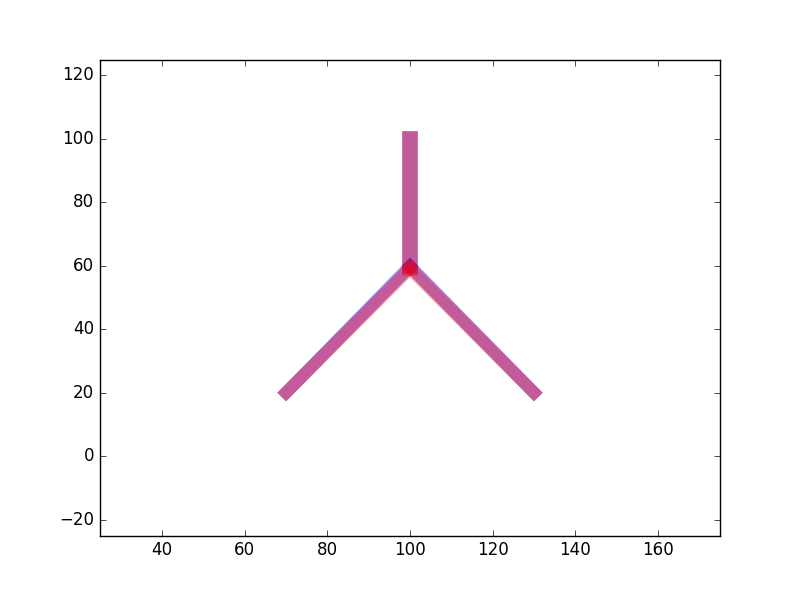
\includegraphics[width=0.45\textwidth]{./Images/Kamiya/Superposition_Firstandlast_t0.png}}
\subfigure[Random child locations and $Q_l = Q_r = \frac{1}{2} Q_p$]{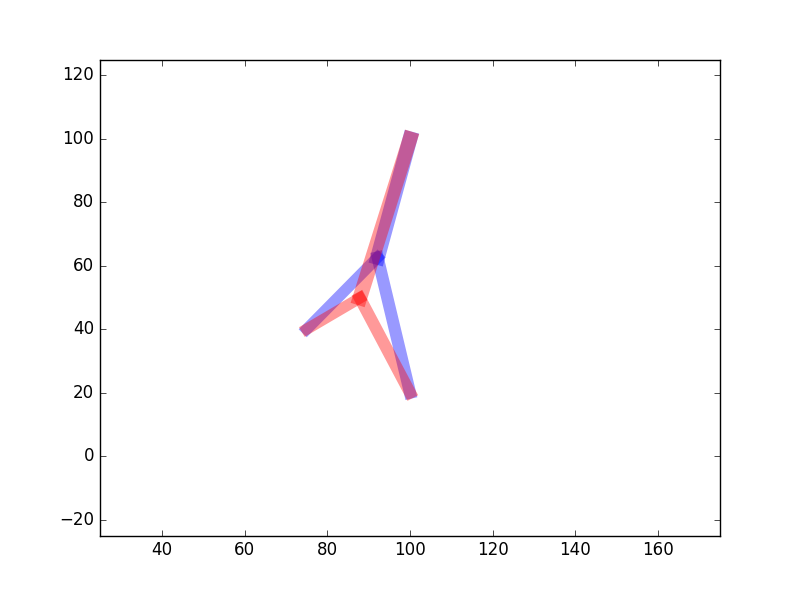
\includegraphics[width=0.45\textwidth]{./Images/Kamiya/Superposition_Firstandlast_t1.png} }\\
\subfigure[$Q_l = \frac{1}{4} Q_p$ and $Q_l = \frac{3}{4} Q_p$]{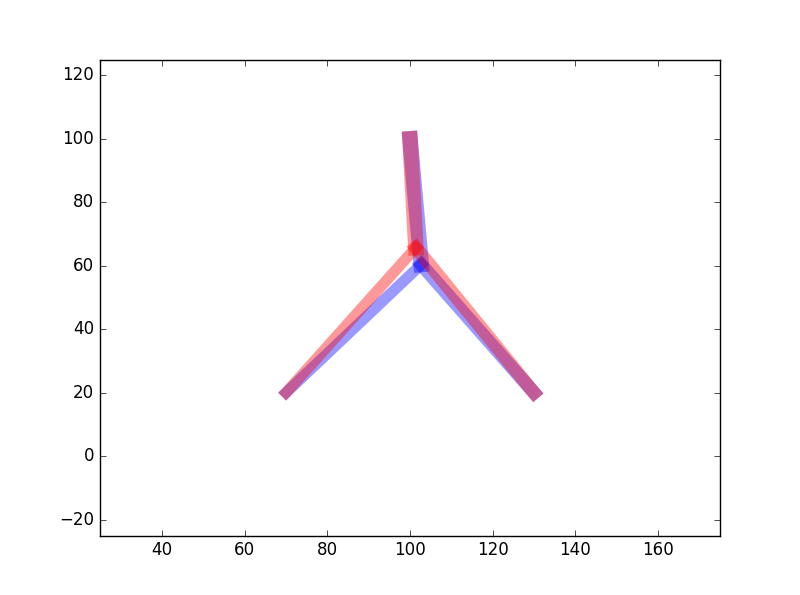
\includegraphics[width=0.45\textwidth]{./Images/Kamiya/Superposition_Firstandlast_t2.png} }
\subfigure[Random child locations and $Q_l = \frac{1}{4} Q_p$, $Q_l = \frac{3}{4} Q_p$]{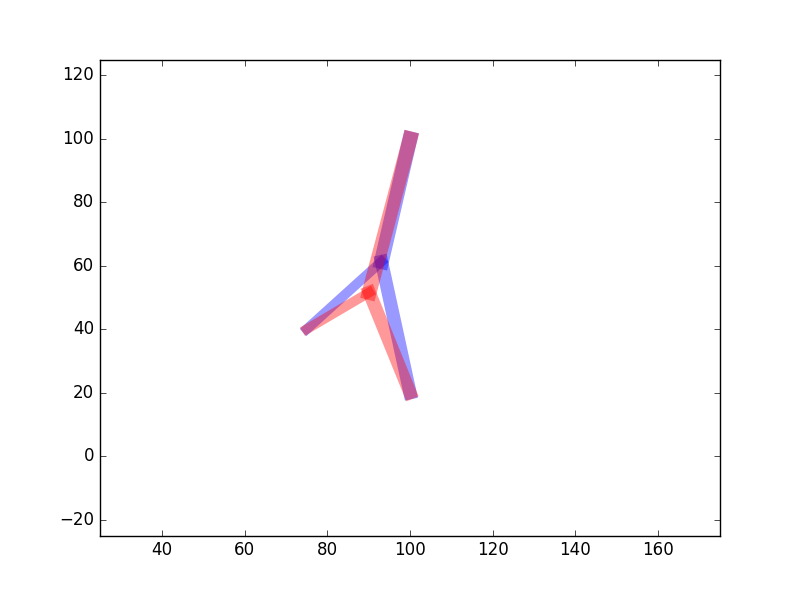
\includegraphics[width=0.45\textwidth]{./Images/Kamiya/Superposition_Firstandlast_t3.png} }

\caption{In blue the starting bifurcation (convex average position), in red the final bifurcation after Kamiya's algorithm reached convergence (tolerance = 0.01). Convergence was reached at 15th, 24th, 31st and 21st iteration respectively in (a),(b),(c),(d). $Q_p$ is the flow in parent branch, $Q_l$ and $Q_r$ are flows in left and right children.}
\label{fig:generation}
\end{figure}

In the figure \ref{fig:generation} (a), for symetric flows and child locations: the optimal bifurcation point corresponds to the convex average.

The figure \ref{fig:generation} (b) illustrates well a Steiner solution to optimal network \cite{bernot2009optimal}: it is more advantageous to transport flows together by delaying bifurcation. In fluid mechanics context, this subadditivity follows from Poiseuille's law, according to which the resistance of a tube increases when it gets thinner.

The figure \ref{fig:generation} (c) shows influence of blood demand on the bifurcation geometry: because flow is more important on the right child, the radius is bigger and the bifurcation is dragged toward this child. Also, we note that the bifurcation is less delayed than for symmetrical flows.

The figure \ref{fig:generation} (d) shows the influence of both destination and demand.


\subsection*{Karch implementation}

Karch added lower and upper bounds to Kamiya's algorithm that ensures:
(1) the bifurcation position within the perfusion volume; (2)
the non degeneracy of the bifurcation (by constraining segment length over segment diameter).


%------------------------------------------------

\section*{Conclusion}

We implemented this CCO method with the same $N_{con}$ and $N_{max}$ as Karch (respectively 20 and 40). The 2D procedure is a good start for debugging, visualizing the results and should be easily convertible into 3D CCO.


We improved computation time by parallelizing the connection test of neighbor segments.

The code is available for 2D and 3D on git hub repo:

 \verb|ClaraJaquet/HeartFlow/SyntheticTreeGeneration_Code|.

\clearpage


\begin{appendices}
\section{Equation \eqref{min volume}, from Kamiya \& Togawa 1972 equation  (6)}\label{appendix:1}
Kamiya uses Murray definition at equation (7) from Physiological principle of minimum work \cite{murray1926physiological} that he calls the simplest requirement for efficiency in the circulation:
\begin{equation*}
f = k r^3
\end{equation*}
with k being a constant, so that the flow of blood past any section shall everywhere bear the same relation to the cube of the radius of the vessel at that point. Using it as:
\begin{equation*}
r_i^3 = \frac{r_i^6 k}{f_i}
\end{equation*}
and combining it this with Murray's law,
\begin{equation*}
r_0^\gamma = r_1^\gamma + r_2^\gamma \text{ with } \gamma = 3
\end{equation*}
 where $r_0$ is the parent radius, $r_1$ and $r_2$ are the children radii, one obtains:
\begin{equation*}
\frac{k r_0^6}{f_0} = \frac{k r_1^6}{f_1} + \frac{k r_2^6}{f_2}
\end{equation*}
that can be simplified into equation \eqref{min volume}.


\section{Equation \eqref{position}, from Kamiya \& Togawa 1972 equation  (7) }\label{appendix:2}

We have
\begin{equation*}
\label{eq:V}
V = \pi(r_0^2 l_0 + r_1^2 l_1 + r_2^2 l_2)
\end{equation*}

and
\begin{align*}
l_0^2 &= \sqlen{0} \\
l_1^2 &= \sqlen{1} \\
l_2^2 &= \sqlen{2} 
\end{align*}

We rewrite \eqref{eq:V}

\begin{equation*}
V = \pi(r_0^2 \sqrt{\sqlen{0}} + r_1^2 \sqrt{\sqlen{1}} + r_2^2 \sqrt{\sqlen{2}})
\end{equation*}

We derive each term with respect to $x$.

\begin{equation*}
\frac{\partial}{\partial x} \sqrt{\sqlen{0}} = \frac{x-x_0}{\sqrt{\sqlen{0}}} = \frac{x-x_0}{l_0},
\end{equation*}
same for the $x_1$ and $x_2$ term, so we have

\begin{equation*}
\frac{\partial V}{\partial x} = \pi\left[ \frac{r_0^2(x-x_0)}{l_0} + \frac{r_1^2(x-x_1)}{l_1} + \frac{r_2^2(x-x_2)}{l_2}\right] = 0
\end{equation*}

Discarding the $\pi$ factor and separating the terms,

\begin{align*}
x\rili{0} + x\rili{1} + x\rili{2} &= x_0\rili{0} + x_1\rili{1} + x_2\rili{2} \\
x(\rili{0} + \rili{1} + \rili{2}) &= x_0\rili{0} + x_1\rili{1} + x_2\rili{2} 
\end{align*}

and thus

\begin{equation*}
x = \frac{x_0\rili{0} + x_1\rili{1} + x_2\rili{2}}{\rili{0} + \rili{1} + \rili{2}}
\end{equation*}

This is one half of Eq.(7) in Kamiya \& Togawa. The other half is obtained by substituting $x$ with $y$ everywhere. This is
formally correct but not 100\% satisfying since the $l_i$ depend on $x$ and $y$.

\end{appendices}

%----------------------------------------------------------------------------------------
%	BIBLIOGRAPHY
%----------------------------------------------------------------------------------------

\bibliographystyle{unsrt}

\bibliography{sample}

%----------------------------------------------------------------------------------------

\end{document}